% !TEX root = ../../main.tex


\begin{figure}[!htb]
\centering
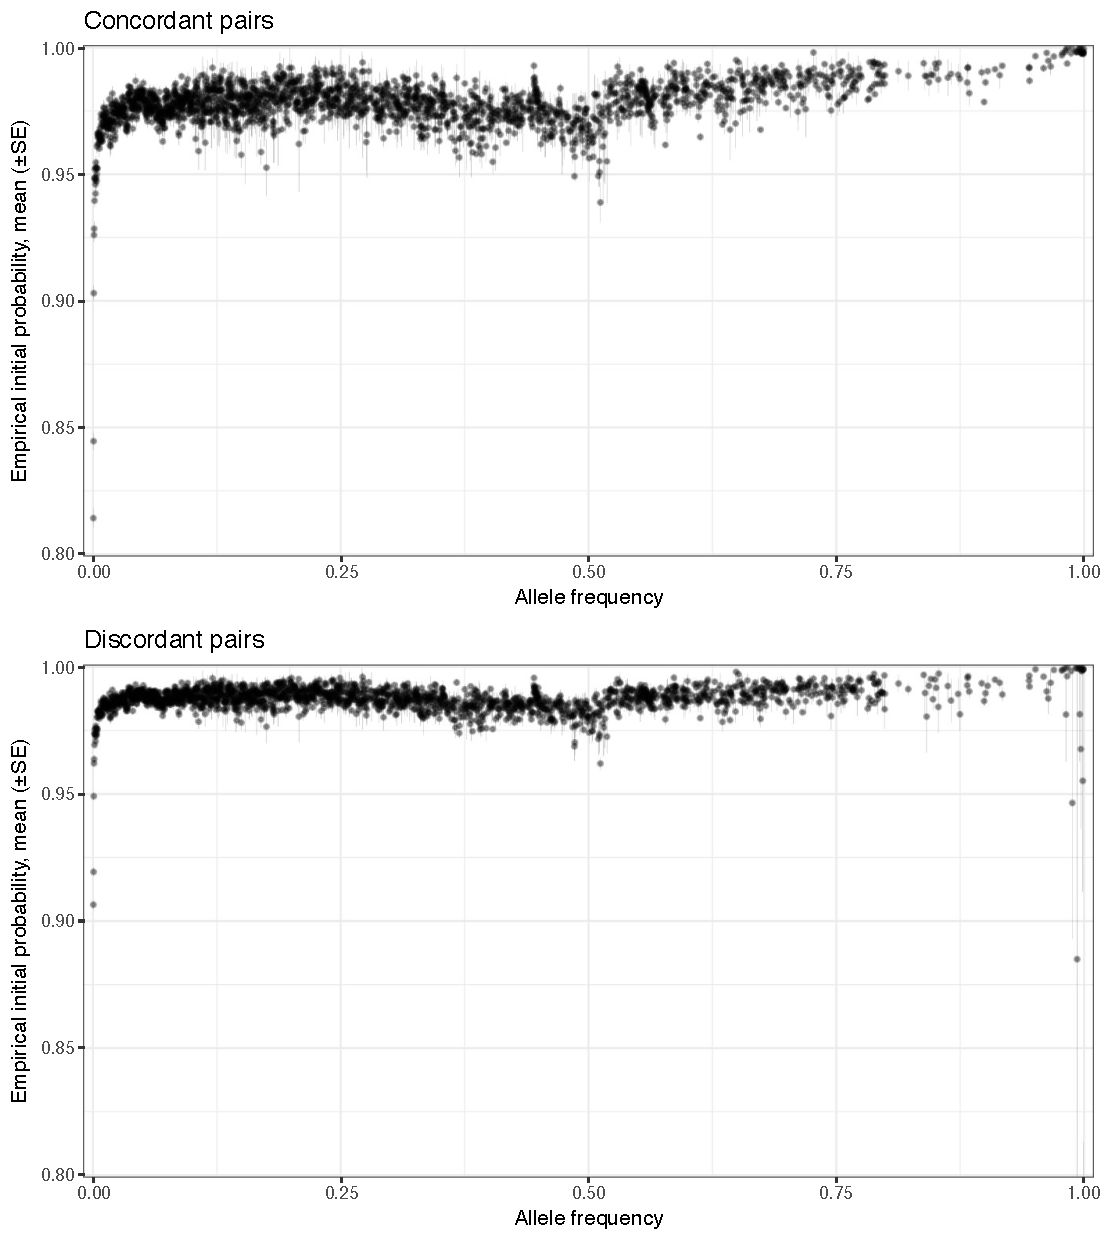
\includegraphics[width=0.66\textwidth]{./img/ch5/hhmm_initial_model_lowres}
\Caption{Empirical initial state probabilities used in the haplotype-based HMM}
{The rate of correctly observing allelic combinations in pairs of haplotypes was measured by comparing data points before and after error, using simulated datasets $\mathcal{D}_B$ and $\mathcal{D}_B^{\ast}$.
At a given focal site, haplotypes were sorted into concordant and discordant pairs as determined from allele sharing in the sample before error.
The allelic state at each pair was then compared to the same location and pair in data after error, to measure the true positive rate of observing the $(1,1)$ allelic combination in concordant pairs and $(0,1)$ in discordant pairs.
Rates are shown as the mean for observations at a given focal allele count ($\pm$SE).
The number of focal sites observed at a specific frequency in the sample differed along the site frequency spectrum, but was capped at a maximum of \n{1000} randomly sampled sites found at a given allele count.}
{fig:hhmm_initial_model}
\end{figure}
